%! TEX root = ../../master.tex
\lecture[TODO]{Di 14 June 2022}{TODO}
\todo{content lec15}

\begin{definition}
    We can generalize matchings as follows:
    \begin{itemize}
        \item Replacing $x(\delta(i)) \leq 1$ by $x(\delta(i)) \leq b$ yields $b$-matchings.
        \item Additionally introducing upper bounds $x_e \leq u_e$ is called $(b,u)$-matching.
    \end{itemize}
\end{definition}
\begin{example}
    A 2-matching is given by
    \vspace{5pt}
    \\
    \begin{minipage}{\textwidth}
        \centering
        \begin{tikzpicture}
            \begin{scope}[every node/.style={circle, draw}]

                \node (1) at (0,0) {};
                \node (2) at (0,2) {};
                \node (3) at (2,0) {};
                \node (4) at (2,2) {};
                \node (5) at (4,2) {};

            \end{scope}
            \path (1.north east) edge (2.south east);
            \path (1.north west) edge (2.south west);
            \path (3) edge (4);
            \path (4) edge (5);
        \end{tikzpicture}
        % \captionof{figure}{A graph with $S$ colored orange}
    \end{minipage}
\end{example}
Notice how perfect $(2,1)$-matchings are close to $\TSP$.
Suppose $S \subseteq V, F \subseteq \delta(S)$ such that $b(S) + u(F)$ is odd.
Further, suppose $b(S)$ is even. Then on one hand, $u(F)$ is odd, on the other hand $x(\delta(S))$ is even.
Then $x(F) \neq x(\delta(S))$. Thus
\begin{align*}
    x(\delta(S) \setminus F) \geq 1 + x(F)-u(F)
\end{align*}
Analoguous, the same follows for $b(S)$ odd.

A perfect $(b,u)$-matching is given by the $\LP$:
\begin{mini*}{x}{c^Tx}{}{}
    \addConstraint{x(\delta(i))}{=b_i, \quad}{\forall i}
    \addConstraint{0}{\leq x \leq u}
    \addConstraint{x(\delta(S)- F)}{\geq 1+ x(F) - u(F), \quad}{\forall S,F \text{ s.t. } b(S)+u(F) \text{ odd}}
\end{mini*}
There is also an equivalent form: \todo{handle teeth stuff}
If $b$ is even, then $b(H)$ is also even.

\begin{align*}
    x(E(H)) + x(T) \leq |H|+ \left\lfloor \frac{|T|}{2}\right\rfloor
\end{align*}

\begin{note}
    For 2-matching, we have exponentially many constraints.
    These can be separated in polynomial time.
    This, however, does \emph{not} mean we can optimize $\TSP$ in polynomial time with Ellipsoid,
    since there could be non-integer optimal solutions (or: we need more constraints, and these make $\TSP$ $\NP$-complete).
\end{note}
\begin{example}
    Consider following part of a 2-matching, where same colors have same edge values in the solution:
    \vspace{5pt}
    \\
    \begin{minipage}{\textwidth}
        \centering
        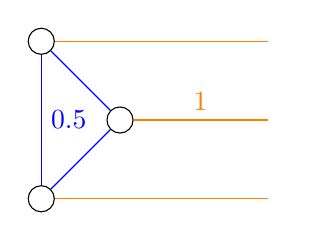
\begin{tikzpicture}
            \begin{scope}[every node/.style={circle, draw}]

                \node (1) at (0,0) {};
                \node (2) at (1,1) {};
                \node (3) at (0,2) {};

            \end{scope}
            \node (1r) at (3,0) {};
            \node (2r) at (3,1) {};
            \node (3r) at (3,2) {};

            \path[blue] (1) edge  (2);
            \path[blue] (2) edge (3);
            \path[blue] (1) edge node[anchor=west] {0.5} (3);
            \path[orange] (1) edge (1r);
            \path[orange] (2) edge node[anchor=south] {1} (2r);
            \path[orange] (3) edge (3r);
        \end{tikzpicture}
        % \captionof{figure}{A graph with $S$ colored orange}
    \end{minipage}
    \\
    \vspace{5pt}
    This violates our handle-teeth constraint for $\TSP$.
\end{example}

\subsection{Fixed dimension $\IP$s}
\begin{theorem}
    For a fixed number of variables, or a fixed number of constraints, there exists a polynomial algorithm that solves $\IP$.
\end{theorem}
\begin{proof}
    The proof requires lattice theory. See \cite[Ch. 2-6.5, Thm.~5.4+5]{int-comb-optimization} for details.
\end{proof}

\subsection{Approximation algorithms}
\begin{recall}
    Greedy on independent systems, which are not matroids, are suboptimal, but can be used for approximated solutions, see \autoref{thm:greedy-bad}.
\end{recall}
\begin{definition}
    For a maximisation problem and (polynomial) algorithm $A$, if
    \begin{align*}
        \max \frac{z^*}{\text{worst-case result of $A$}} \leq \alpha
    \end{align*}
    we call $A$ an \vocab{$\alpha$-approximation} algorithm.
\end{definition}
\begin{example}
    Matching can be solved by Greedy as a $2$-approximation.
\end{example}
\begin{definition}
    There exist several classes of approximation algorithms:
    \begin{itemize}
        \item $\FPTAS$ (\vocab[approximation!FPTAS]{Fully Polynomial Time Approximation Scheme}):
              There exists an algorithm polynomial in $|I|$ and $1/ \eps$ to get an $(1+\eps)$-approximation.
        \item $\PTAS$ (\vocab[approximation!PTAS]{Polynomial Time Approximation Scheme}):
              There exists an algorithm polynomial in $|I|$ and potentially exponential in $1/ \eps$ to get an $(1+\eps)$-approximation.
        \item \vocab[approximation!fixed factor]{Fixed Factor}: There exists a threshold $\beta$
              such that there is a polynomial algorithm for all $\alpha \geq \beta$, but it is $\NP$-hard
              to approximate for $1\leq \alpha < \beta$.
        \item Inapproximate $\NP$-hard to approximate for any $\alpha > 1$.
    \end{itemize}
\end{definition}
\todo{what does this mean? Inapproximate}

\subsection{Rounding non-integer solutions}
\begin{idea}
    Solve $\LP$, get $x^{\LP}$, and round up or down to get a solution $x^{\IP}$.
\end{idea}
This is a bad idea in general:
\begin{theorem}
    Naive rounding of $x^{\LP}$ can introduce arbitrarily large errors
    (see \cite[Thm.~5.7]{comb-optimization-korte} for a more exact version).
\end{theorem}
\begin{proof}
    We can construct following bad instance depending on some parameter $\alpha$,
    such that the gap between the rounded optimal $\LP$ solution and the actual optimal $\IP$ solution scales with $\alpha$.
\end{proof}
\todo{lattice plot}
\begin{remark}
    Not all instances can be rounded out-of-the-box to a feasible solution.
\end{remark}
\todo{sharp triangle plot non-roundable}

\subsection{Cutting Planes}
Recall our initial idea was to compute the integer hull $P^I$ of $P$, which is however $NP$-hard.
But, instead of computing \emph{all} of $P^I$, in most cases it suffices to calculate $P^I$ "near" $x^I$.
Thus, we want to find a cutting plane $\alpha^Tx > \beta$ such that
\begin{enumerate}
    \item $x^{\LP}$ violates the plane, i.e. $\alpha^T x^{\LP} > \beta$, and
    \item all of $P^I$ satisfies the cutting plane,
          i.e. for all $x \in P \cap \integers^n$ should hold $\alpha^T x^{\LP} \leq \beta$
\end{enumerate}
\begin{idea}
    Find Cutting Planes, add to $\LP$ (reoptimize via dual simplex), and repeat until we get $x^{\IP}$.
\end{idea}
Finding cutting planes can be done via $\SEP$.
\begin{remark}
    There is a technical issue with convergence. While we know, in general we cannot guarantee polynomial running time,
    it is also possible that $P^I$ isn't even a polyhedron:

    Because of $\sqrt{2}$ being irrational, there will be infinitely feasible integer points
    getting infinitely close, but never touching it. This cannot be handled with finitely many constraints.
\end{remark}
\todo{plot irrational constraint}
\begin{theorem}[Fundamental theorem of $\IP$]
    For rational $A,b$ and $P=\{x \mid Ax \leq b\}$ holds that $P^I$ is a polyhedron.
\end{theorem}
\begin{proof}
    See \cite[Thm.~5.1]{comb-optimization-korte}
\end{proof}